\documentclass[11pt]{article}
\usepackage[scaled=0.92]{helvet}
\usepackage{geometry}
\geometry{letterpaper,tmargin=1in,bmargin=1in,lmargin=1in,rmargin=1in}
\usepackage[parfill]{parskip} % Activate to begin paragraphs with an empty line rather than an indent %\usepackage{graphicx}
\usepackage{amsmath,amssymb, mathrsfs, dsfont}
\usepackage{tabularx}
\usepackage[font=footnotesize,labelfont=bf]{caption}
\usepackage{graphicx}
\usepackage{xcolor}
%\usepackage[linkbordercolor ={1 1 1} ]{hyperref}
%\usepackage[sf]{titlesec}
\usepackage{natbib}
\usepackage{../../Tianpei_Report}
%\usepackage{appendix}
%\usepackage{algorithm}
%\usepackage{algorithmic}

%\renewcommand{\algorithmicrequire}{\textbf{Input:}}
%\renewcommand{\algorithmicensure}{\textbf{Output:}}



\begin{document}
\title{Lecture 4: Variational Inference in Exponential Family Graphical Models}
\author{ Tianpei Xie}
\date{Aug. 25th., 2022 }
\maketitle
\tableofcontents
\newpage
\allowdisplaybreaks
\section{Background knowledge}
Recall the formulation of Bayesian network and Markov network
\begin{itemize}
\item Given directed graph $\cG=(\cV, \cE)$, where $(s,t) \neq (t,s)$, the \textbf{directed graphical model}  factorizes the joint distribution into a set of \emph{factors} $\{p_s(x_s | x_{\pi(s)}): s\in \cV\}$ according to the ancestor relations defined in $\cG$
\begin{align}
p(x_1, \ldots, x_{m}) &= \prod_{s \in \cV}p_s(x_s | x_{\pi(s)}). \label{eqn: dag_graph_factorization}
\end{align} This class of models are also referred as \emph{\textbf{Bayesian networks}} \citep{koller2009probabilistic}.


\item Given undirected graph $\cG=(\cV, \cE)$, where $(s,t) = (t,s)$, the joint distribution of \textbf{Markov random fields} (\textbf{Markov network}) \emph{factorize} as
\begin{align}
p(x_1, \ldots, x_{m}) &= \frac{1}{Z}\prod_{C \in \cC}\psi_{C}(x_{C}),\label{eqn: mrf_graph_factorization}
\end{align} where $Z$ is a constant chosen to ensure that the distribution is normalized. The set $\cC$ is often taken to be the \emph{set of all \textbf{maximal cliques} of the graph}, i.e., the set of cliques that are \emph{not} properly contained within any other clique. Note that any representation based on nonmaximal cliques can always be converted to one based on maximal cliques by redefining the compatibility function on a maximal clique to be the \emph{product} over the compatibility functions on the \emph{subsets} of that clique.

\item The canonical representation of \underline{\emph{\textbf{exponential famlity}}} of distribution has the following form
\begin{align}
p(x_1, \ldots, x_{m}) = p(\mb{x}; \mb{\eta}) &= \exp\paren{\inn{\mb{\eta}}{\mb{\phi}(\mb{x})} - A(\mb{\eta})}h(\mb{x})\nu(d\mb{x}) \nonumber \\
&= \exp\paren{\sum_{\alpha}\eta_{\alpha}\phi_{\alpha}(\mb{x}) -  A(\mb{\eta})} \label{eqn: exp_fam}
\end{align} where $\phi$ is a feature map  and $\mb{\phi}(\mb{x})$ defines a set of \emph{\textbf{sufficient statistics}} (or \emph{\textbf{potential functions}}). The normalization factor is defined as
\begin{align*}
 A(\mb{\eta}) &:= \log \int \exp\paren{ \inn{\mb{\eta}}{\mb{\phi}(\mb{x})} }h(\mb{x})\nu(d\mb{x}) = \log Z(\mb{\eta})
\end{align*} $A(\mb{\eta})$ is also referred as \textbf{\emph{log-partition function}} or \emph{cumulant function}. The parameters $\mb{\eta} = (\eta_{\alpha})$ are called \textbf{\emph{natural parameters}}  or \emph{canonical parameters}. The canonical parameter $\set{\eta_{\alpha}}$ forms a \textbf{natural (canonical) parameter space}
\begin{align}
\Omega = \set{\mb{\eta} \in \bR^{d}: A(\mb{\eta}) < \infty} \label{eqn: canonical_space}
\end{align}

\item The exponential family is the unique solution of \textbf{\emph{maximum entropy estimation}} problem:
\begin{align}
\min_{q \in \Delta}&\quad \kl{q}{p_{0}} \label{eqn: max_ent}\\
\text{s.t.}&\quad \E{q}{\phi_{\alpha}(X)} = \mu_{\alpha}\,\quad  \forall\, \alpha \in \cI   \label{eqn: max_ent_mean_constraint}
\end{align} where $\kl{q}{p_0} = \int \log(\frac{q}{p_0}) q dx = \E{q}{\log\frac{q}{p_0}}$ is the relative entropy or the Kullback-Leibler divergence of $q$ w.r.t. $p_0$.

Here $\mb{\mu} = (\mu_{\alpha})_{\alpha \in \cI}$ is a set of  \textbf{\emph{mean parameters}}. The space of mean parameters $\cM$ is a \emph{convex polytope} spanned by potential functions $\set{\phi_{\alpha}}$.
\begin{align}
\cM &:= \set{\mb{\mu} \in \bR^d: \exists q\,\; \text{s.t. } \E{q}{\phi_{\alpha}(X)} = \mu_{\alpha}\,\quad  \forall\, \alpha \in \cI} = \text{conv}\set{\phi_{\alpha}(x),\; x\in \cX, \;\alpha \in \cI}  \label{eqn: marginal_polytope}
\end{align}

\item Note that $A(\mb{\eta})$ is a convex function and its gradient $\grad{}{A}: \Omega \rightarrow \cM^{\circ}$ is a bijection between the natural parameter space $\Omega$ and the \underline{\textbf{interior}} of $\cM$,  $\cM^{\circ}$; $\grad{}{A}(\mb{\eta}) = \mb{\mu}$ based on the following equation 
\begin{align}
\partdiff{A}{\eta_{\alpha}} &= \E{\mb{\eta}}{\phi_{\alpha}(X)} := \int_{\cX^{m}}\phi_{\alpha}(\mb{x}) q(\mb{x}; \mb{\eta}) d\mb{x} = \mu_{\alpha} \label{eqn: partition_first_order}
\end{align}

\item Moreover $A(\mb{\eta})$ has a variational form 
\begin{align}
A(\mb{\eta}) &=  \sup_{\mb{\mu} \in \cM}\set{ \inn{\mb{\eta}}{\mb{\mu}} - A^{*}(\mb{\mu})} \label{eqn: log_partition_variational_form}
\end{align}
where $A^{*}(\mb{\mu})$ is the conjugate dual function of $A$ and it is defined as
\begin{align}
A^{*}(\mb{\mu}) &:= \sup_{\mb{\eta} \in \Omega} \set{\inn{\mb{\mu}}{\mb{\eta}} - A(\mb{\eta})} \label{eqn: conjugate_dual_partition}
\end{align}

It is shown that $A^{*}(\mb{\mu})  = -H(q_{\mb{\eta}(\mb{\mu})})$ for $\mb{\mu} \in  \cM^{\circ}$ which is the negative entropy. $A^{*}(\mb{\mu})$ is also the optimal value for the \textbf{maximum likelihood estimation} problem on $p$. The exponential family can be reparameterized according to its mean parameters $\mb{\mu}$ via backward mapping $(\grad{}{A})^{-1}: \cM^{\circ} \rightarrow  \Omega$, called \textbf{mean parameterization}.

\item We can formulate the \textbf{KL divergence} between two distributions in exponential family $\Omega$ using its primal and dual form
\begin{itemize}
\item \textbf{Primal-form}: given $\mb{\eta}_1, \mb{\eta}_2 \in \Omega$
\begin{align}
\kl{p_{\mb{\eta}_1}}{p_{\mb{\eta}_2}} \equiv  \kl{\mb{\eta}_1}{\mb{\eta}_2}
&=  A(\mb{\eta}_2) - A(\mb{\eta}_1) -  \inn{\mb{\mu}_{1}}{\mb{\eta}_2 - \mb{\eta}_1}  \label{eqn: kl_primal}\\
&\equiv  A(\mb{\eta}_2) - A(\mb{\eta}_1) -  \inn{\grad{}{A}(\mb{\eta}_1)}{\mb{\eta}_2 - \mb{\eta}_1}  \nonumber
\end{align}

\item \textbf{Primal-dual form}: given $\mb{\mu}_1 \in \cM, \mb{\eta}_2 \in \Omega$
\begin{align}
 \kl{\mb{\mu}_1}{\mb{\eta}_2} &= A(\mb{\eta}_2) + A^{*}(\mb{\mu}_1) - \inn{\mb{\mu}_{1}}{\mb{\eta}_2}  \label{eqn: kl_primal_dual}
\end{align}

\item \textbf{Dual-form}: given $\mb{\mu}_1, \mb{\mu}_2  \in \cM$
\begin{align}
 \kl{\mb{\mu}_1}{\mb{\mu}_2} &= A^{*}(\mb{\mu}_1) - A^{*}(\mb{\mu}_{2}) - \inn{\mb{\eta}_2}{\mb{\mu}_{1} - \mb{\mu}_{2}}  \label{eqn: kl_dual} \\
 &\equiv  A^{*}(\mb{\mu}_1) - A^{*}(\mb{\mu}_{2}) - \inn{\grad{}{A^{*}}(\mb{\mu}_{2})}{\mb{\mu}_{1} - \mb{\mu}_{2}} \nonumber
\end{align}
\end{itemize}


\item The exact inference on \textbf{tree-based models} makes use of the \textbf{decomposition} property of tree, $\cT = (\cV, \cE_{\cT})$. Specifically, define the neighborhood of node $s$ as
\begin{align*}
\cN(s) &= \set{t\in \cV: (s,t) \in \cE_{\cT} }
\end{align*} For each $u \in \cN(s)$, let $\cT_u = (\cV_u, \cE_u)$ be the subgraph formed by the set of nodes (and edges joining them) that \emph{can be reached from} $u$ by \textbf{paths} that \emph{\textbf{do not pass}} through node $s$. An \textbf{important property} for tree is that the subgraph $\cT$ is a tree and  for any $u\neq t,  \forall u,t \in \cN(s)$, $\cT_{u} \cap \cT_{t} = \emptyset$.  This means that we can \textbf{decompose} the tree $\cT_{s}$ rooted at $s$, by \textbf{removing} $s$ from the tree. It then form a collection or non-overlapping subtrees $\{\cT_t, t \in \cN(s)\}$.

\item The tree-based Markov random field is defined as 
\begin{align}
p(x_1, \ldots, x_{m}; \cT) &= \frac{1}{Z}\prod_{s\in \cV}\psi_{s}(x_{s})\prod_{(s,t) \in \cE_{\cT}}\psi_{s,t}(x_{s}, x_{t}), \label{eqn: mrf_tree_factorization}
\end{align}

\item The \textbf{\emph{Belief Propagation algorithm}} is based on \emph{dynamic programming}. The key is to pass \emph{messages} from one node to its neighborhood carrying marginalized probability from other nodes. \emph{\textbf{Message}} is a value function, which is defined as 
\begin{align}
M_{t \rightarrow s}^{*}(x_s) := M_{t,s}^{*}(x_s) &= \sum_{\mb{x}_{\cV_{t}}}p_{t}(\mb{x}_{\cV_{t}}|x_s; \cT_{t})
= \sum_{\mb{x}_{\cV_t}}\psi_{s,t}(x_s, x_t)p(\mb{x}_{\cV_t}; \cT_{t})  \label{eqn: mrf_tree_sum_product_message} 
\end{align}
The target is to find marginal distribution at $x_s$
\begin{align}
\mu_{s}(x_{s}) &:= \sum_{\mb{x}_{-s}}p(x_s, \mb{x}_{-s}) \nonumber\\
&=\psi_{s}(x_s)\prod_{t \in \cN(s)}M_{t,s}^{*}(x_s). \label{eqn: mrf_tree_sum_product_marginal} 
\end{align}
The sum-product algorithm is based on the following \emph{\textbf{Bellman equation}}:
\begin{align}
M_{t,s}^{*}(x_s) &= \sum_{\mb{x}_{\cV_t}}\psi_{s,t}(x_s, x_t)p(\mb{x}_{\cV_t}; \cT_{t}) \nonumber\\
&= \kappa \sum_{x_t \in \cX}\set{\psi_{s,t}(x_s, x_t)\psi_{t}(x_t)\prod_{u \in \cN(t) - \set{s}}M_{u,t}^{*}(x_t)}, \,  \forall t\in \cN(s),  s \in \cV \label{eqn: mrf_tree_sum_product_bellman_equation}
\end{align} where $\kappa > 0$ again denotes a \emph{normalization constant}. 

\end{itemize}

\newpage
\section{Approximate inference via variational methods}
The message passing algorithms in \eqref{eqn: mrf_tree_sum_product_bellman_equation} are mainly for tabular-based graphical model. For graphical model using function representation, such as those in exponential families, exact inference task is challenging. In these graphical models, two fundamental difficulties associated with:
\begin{itemize}
\item the nature of the \textbf{constraint set} $\cM$, which is high dimensional with many facets and extreme points; 

\item the lack of an explicit form for the \textbf{dual function} $A^{*}$, esp. \textbf{the negative entropy} on joint distribution cannot be decomposed according to graph $\cG$.
\end{itemize} 
Therefore, we focus on \textbf{approximate Inference methods} of exponential family graphical model. There are two main branches:
\begin{itemize}
\item \underline{\textbf{\emph{Monte Carlo sampling methods}}}: Many graphical models have explicit function form for \emph{conditional probability} (e.g. \emph{Gaussian graphical model}, \emph{LDA}, \emph{RBMs} etc.). This allows us to apply sampling techiques such as \emph{importance sampling}, \emph{Gibbs sampling}, \emph{stimulated annealing}, \emph{hybrid Monte Carlo} etc. \citep{liu2001monte, shapiro2003monte}. The \textbf{key idea} behind sampling based inference methods is that the high dimensional integration can be \emph{\textbf{approximated}} via \emph{\textbf{sample average}} of some statistics. Each factor can be used as a generator on a small number of variables based on local information. The \textbf{drawbacks} include \textbf{randomness of solutions}, \textbf{slow convergence}, \textbf{high variance} etc. 

\item \underline{\textbf{\emph{Variational inference methods}}}: Variational inference methods are based on the \textbf{\emph{variational principle}} of log-partition function \eqref{eqn: log_partition_variational_form} and conjugate duality between $A$ and $A^{*}$.  Unlike the \emph{stochastic methods} above, these methods are \textbf{\emph{deterministic}}. We mainly discuss two classes of metheds
\begin{itemize}
\item The \emph{belief propagation} based on \underline{\textbf{\emph{Bethe variational problem (BVP)}}}. It relaxes the constraint set from $\cM(\cG)$ to a \emph{convex} polytope $\cL(\cG)$ and then approximates the entropy using \emph{Bethe entropy approximation}. Both approximations allow the problem to be factorized according to graph topology. 

\item The \underline{\textbf{\emph{mean field methods}}}. These methods limit the distributions within an \emph{non-convex set} $\cM_{\cF} \subseteq \cM$ on \emph{tractable graph} $\cF$, e.g. fully factorized. They find the closet tractable model in exponential family that satisfy the mean matching conditions.
\end{itemize} These methods reach the \emph{entropy decomposition} at the expense of \textbf{\emph{losing convexity}} in the problem formulations. For BVP, the objective function is non-convex. For the mean field method, the feasible region is non-convex.  
\end{itemize}





\section{Belief propagation for exponential families}\label{sec: bp}
Unlike tabular methods, exponential families are defined \emph{\textbf{globally}} by joint distributions. In order for the belief propagation to work, we need to break it down into a set of local factors  and consider the local objective functions on each factor. In this section, we will
\begin{itemize}
\item \textbf{Relax} the constraint set from (global) marginal polytope $\cM(\cG)$ to $\cL(\cG)$ as a set of \textbf{pseudo-marginal} distributions within each factors

\item \textbf{Approximate} the global entropy $-A^{*}(\tau)$  by \textbf{Bethe entropy} which can be \textbf{decomposed} into entropies on each local factors 
\end{itemize}

\subsection{Approximate $\cM(\cG)$ via pseudo-marginal distributions}
\begin{figure}
\begin{minipage}[t]{1\linewidth}
  \centering
  \centerline{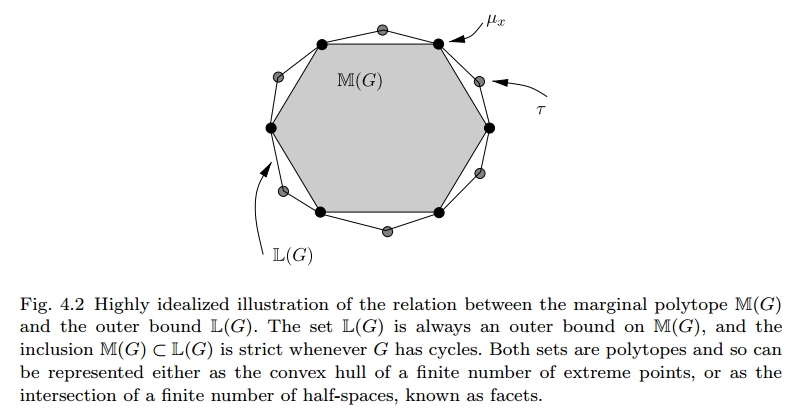
\includegraphics[scale = 0.5]{outbound_marginal.png}}
\end{minipage}
\caption{\footnotesize{\textbf{The marginal polytope $\cM(\cG)$ and its outer bound relaxation $\cL(\cG)$.}}}
\label{fig: outbound_marginal}
\end{figure}


Consider the pairwise Markov random fields with binary indicator potential functions: 
\begin{align}
\phi_{s;j}(x_s) &= \ind{x_s = j}  \label{eqn: metric_label_sufficient}
\end{align} 
Moreover, for each edge $(s,t)$ and pair of values $(j,k) \in \cX \times \cX$ , define the sufficient statistics
\begin{align}
\phi_{st;jk}(x_s, x_t) &= \ind{x_s = j \, \land x_{t} = k}  \label{eqn: metric_label_sufficient2}
\end{align}
The joint distribution is 
\begin{align}
p(x_1, \ldots, x_m; \mb{\eta}) &= \exp\paren{\sum_{s\in \cV}\sum_{j \in \cX}\eta_{s;j}\,\phi_{s;j}(x_s)  + \sum_{(s,t) \in \cE}\sum_{(j,k) \in \cX \times \cX}\eta_{st;jk}\,\phi_{st;jk}(x_s, x_t)  - Z(\mb{w})}, \label{eqn: potts_model}
\end{align}

As discussed before, the mean parameter space $\cM(\cG)$ is the \emph{\textbf{marginal polytope}} over $\cG$ since 
\begin{align*}
\cM(\cG) &:= \set{\mb{\mu} \in \bR^d: \exists q\,\; \text{s.t. } \E{q}{\phi_{\alpha}(X)} = \mu_{\alpha}\,\quad  \forall\, \alpha \in \cI} \\
\text{where }&\E{p}{ \ind{x_s = j \, \land x_{t} = k}} = \mu_{st;jk} = \bP(X_s = j \land X_t = k), \quad \forall s,t, j, k \\
&\E{p}{  \ind{x_s = j} } = \mu_{s;j} = \bP(X_s = j ),  \quad \forall s, j
\end{align*} defines a set of matching constraints on the marginal distribution of $p$ within each factor.  

As a convex set, $\cM(\cG)$ can be represented as \emph{intersection of a finite number of half spaces}, which usually does not have explicit form. Therefore we consider an \textbf{outer bound set} $\cL(\cG)$ as its \textbf{relaxation}:
\begin{align}
\cL(\cG) &= \set{\mb{\tau} > 0:  \tau_s \text{ satisfies \eqref{eqn: local_normalization_constraints}}\; \forall s\in \cV, \; \tau_{s,t}\text{ satisfies \eqref{eqn: local_marginalization_constraints}}\; \forall (s,t) \in \cE} \label{eqn: dual_marginal_polytope}\\
&\sum_{x_s \in \cX}\tau_{s}(x_s) = 1,  \quad \forall s \in \cV \label{eqn: local_normalization_constraints}\\
&\sum_{x_t' \in \cX}\tau_{s,t}(x_s, x_t') = \tau_{s}(x_s), \quad \forall x_s, x_t \in \cX, \, (s,t) \in \cE  \label{eqn: local_marginalization_constraints}\\
&\sum_{x_s' \in \cX}\tau_{s,t}(x_s', x_t) = \tau_{t}(x_t). \nonumber
\end{align} The $\cL(\cG)$  are set of marginal distributions that fit the \textbf{\emph{local consistent requirement}} since they only consider the distribution\textbf{\emph{within each factor}} but the entire joint distribution.  Note that $\cL(\cG)$ is defined by $O(|\cV| + |\cE|)$ linear constraints. On the other hand, $\cM(\cG)$ has a total of $|\cX^m|$ extreme points.

The construction of $\cL(\cG)$ follows a \underline{\textbf{\emph{bottom-up}}} approach, i.e. focusing on finding consistent marginal distributions just \emph{\textbf{within each local factor}}. On the other hand, the marginal polytope $\cM(\cG)$ is constructed via a \emph{\textbf{top-down approach}}, i.e. it begins with \textbf{joint distribution} $p$ and then \emph{marginalize} over other variables to obtain the marginal distribution within each factor. It is easy to see that $\cM$ follows the local consistency conditions in $\cL$ but not vice versa.

\begin{proposition}
The inclusion $\cM(\cG) \subseteq \cL(\cG)$ holds for any graph. For a tree-structured graph $\cT$ , the marginal polytope $\cM(\cT)$ is equal to $\cL(\cT)$.
\end{proposition} 

For tree structures $\cL(\cG) = \cM(\cG)$, $\mb{\tau} \in \cL(\cG)$ defined a valid marginal distribution. But for graphs with circles, they are not \emph{valid} marginal distribution, i.e. $\tau_{s,t} \neq \sum_{-\{s,t\}}p(\mb{x})$. In this case, they are called \textbf{\emph{pseudo-marginals}}.
\subsection{Bethe entropy approximation}
The  entropy $-A^{*}$ usually does not have closed-form expression. One exception is tree-structured graph $\cT$. 
\begin{align}
-A^{*}(\mb{\mu})  &= H(p_{\mb{\mu}}) = \E{\mb{\mu}}{-\log p_{\mb{\mu}}(X)} \nonumber\\
&= \sum_{s \in \cV}H_{s}(\mu_{s}) - \sum_{(s,t) \in \cE}I(\mu_{s,t}) \label{eqn: entropy_decomposition}
\end{align} where $\mu_{s}$ and $\mu_{s,t}$ are set of marginal distributions defined in $\cM(\cT)$. The total entropy $-A^{*}$ is decomposed into  \textbf{\emph{node entropies}} and \textbf{\emph{edge mutual information}} within each factor. These quantities are defined as below: 
\begin{align}
H_{s}(\mu_{s}) &= \E{\mu_{s}}{- \log \mu_{s}} = \int_{\cX} - \mu_{s}(x_s) \log \mu_{s}(x_s) d x_s, \quad \forall s\in \cV \label{eqn: node_entropy}\\
I(\mu_{s,t}) &= \E{\mu_{s,t}}{\log \frac{\mu_{s,t}}{\mu_{s} \mu_{t}}} = \int_{\cX\times \cX}\mu_{s,t}(x_s, x_t) \log\paren{\frac{\mu_{s,t}(x_s, x_t)}{\mu_{s}(x_s) \mu_{t}(x_t)}} d x_s d x_t, \; \forall (s,t) \in \cE \label{eqn: edge_mutual_information}
\end{align}

For graphs with cycles, the decomposition \eqref{eqn: entropy_decomposition} is seen as an approximation of $H(p_{\mb{\mu}})$, called \textbf{\emph{Bethe entropy approximation}}, i.e.
\begin{align}
H(\tau) &\approx H_{Bethe}(\tau) :=  \sum_{s \in \cV}H_{s}(\tau_{s}) - \sum_{(s,t) \in \cE}I(\tau_{s,t})  \label{eqn: bethe_entropy_approximation}
\end{align}
An important fact, \textbf{central} in the derivation of the sum-product algorithm, is that this approximation \eqref{eqn: bethe_entropy_approximation} can be evaluated for any set of \emph{\textbf{pseudomarginals}} $\{\tau_s , s \in  \cV \}$ and $\{\tau_{s,t}, (s,t ) \in \cE\}$ that belong to $\cL(\cG)$. 

Now we can formulate the \underline{\emph{\textbf{Bethe variational problem (BVP)}}}:
\begin{align}
\max_{\mb{\tau} \in \cL(\cG)}& \inn{\mb{\tau}}{\mb{\eta}} +  \sum_{s \in \cV}H_{s}(\tau_{s}) - \sum_{(s,t) \in \cE}I(\tau_{s,t}) \label{eqn: bethe_variational_problem}
\end{align} The objective function is called \emph{\textbf{Bethe free energy}}. This problem has a very simple structure: the cost function is given in \textbf{\emph{closed form}}, it is \textbf{\emph{differentiable}}, and the constraint set $\cL(\cG)$ is a polytope specified by a \emph{small number of constraints}. Due to its simple form and the fact that $H_{Bethe}(\tau)$ factorizes over $\cG$, we can solve \eqref{eqn: bethe_variational_problem} efficiently via \textbf{belief propagation} (\emph{sum-product algorithm}). 

\subsection{Sum-product for Bethe variational problem}
Let us formulate the (partial) Lagrangian function for BVP:
\begin{align}
\cL(\mb{\tau}, \mb{\lambda}; \mb{\eta}) &:=  \inn{\mb{\tau}}{\mb{\eta}} +  \sum_{s \in \cV}H_{s}(\tau_{s}) - \sum_{(s,t) \in \cE}I(\tau_{s,t}) +\sum_{s\in \cV} \lambda_{ss}\brac{ \sum_{x_s \in \cX}\tau_{s}(x_s) - 1} \nonumber\\
& + \sum_{(s,t) \in \cE}\set{\sum_{x_s}\lambda_{t,s}(x_s)\brac{\tau_{s}(x_s) - \sum_{x_t \in \cX}\tau_{s,t}(x_s, x_t) } + \sum_{x_t}\lambda_{s,t}(x_t)\brac{\tau_{t}(x_t) - \sum_{x_s \in \cX}\tau_{s,t}(x_s, x_t) }} \label{eqn: lagrangian_bvp}
\end{align}

We have the following theorem which tells that sum-product is the algorithm to solve \eqref{eqn: lagrangian_bvp}.
\begin{theorem} (\textbf{Sum-Product} and the \textbf{Bethe Problem}) \citep{wainwright2008graphical}. \\
The \underline{sum-product updates} are a Lagrangian method for attempting to solve the \textbf{Bethe variational problem}:
\begin{enumerate}
\item For any graph $\cG$, any fixed point of the sum-product updates specifies a pair $(\mb{\tau}^{*}, \mb{\lambda}^{*})$ such that
\begin{align}
\grad{\mb{\tau}}{\cL(\mb{\tau}^{*}, \mb{\lambda}^{*}; \mb{\eta})} = \mb{0} \;\text{ and } \;
\grad{\mb{\lambda}}{\cL(\mb{\tau}^{*}, \mb{\lambda}^{*}; \mb{\eta})} = \mb{0}. \label{eqn: sum_product_bethe_variational_cond}
\end{align}

\item For a \underline{\textbf{tree-structured}} Markov random field (MRF), the Lagrangian Equations \eqref{eqn: sum_product_bethe_variational_cond} have a \textbf{unique solution} $(\mb{\tau}^{*}, \mb{\lambda}^{*})$,  where the elements of $\mb{\tau}^{*}$ correspond to the \textbf{exact} \emph{singleton} and \emph{pairwise marginal distributions} of the MRF. Moreover, the \textbf{optimal value} of the BVP is equal to the cumulant function $A(\mb{\eta})$.
\end{enumerate}
\end{theorem}
\begin{proof} We just prove the first part. The second part see \citep{wainwright2008graphical}. Computing $\grad{\mb{\lambda}}{\cL(\mb{\tau}^{*}, \mb{\lambda}^{*}; \mb{\eta})} = \mb{0}$ results in the marginalization and normalization constraint \eqref{eqn: local_marginalization_constraints} and \eqref{eqn: local_normalization_constraints}. 
Computing $\grad{\mb{\tau}}{\cL(\mb{\tau}^{*}, \mb{\lambda}^{*}; \mb{\eta})} = \mb{0}$ results in 
\begin{align*}
0=\grad{\mb{\tau}}{\cL(\mb{\tau}^{*}, \mb{\lambda}^{*}; \mb{\eta})}\big|_{s, x_s} &= \eta_{s}(x_{s}) - \log \tau_{s}(x_{s}) + \lambda_{ss}+ \sum_{t \in \cN(s)}\lambda_{t,s}(x_s) \\
0=\grad{\mb{\tau}}{\cL(\mb{\tau}^{*}, \mb{\lambda}^{*}; \mb{\eta})}\big|_{(s,t), x_s, x_t} &= \eta_{s,t}(x_{s}, x_{t}) - \log \tau_{s,t}(x_s, x_t)  \\
&+ \log\tau_{s}(x_{s}) +  \log\tau_{t}(x_{t})- \lambda_{t,s}(x_s) - \lambda_{s,t}(x_t)
\end{align*} Note  that constant terms are absorbed by the slack variable for the positiveness constraint.
Thus
\begin{align}
\log \tau_{s}(x_{s}) &=  \eta_{s}(x_{s}) + \lambda_{ss}+ \sum_{t \in \cN(s)}\lambda_{t,s}(x_s) \label{eqn: bethe_node_psuduomargin} \\
 \log \tau_{s,t}(x_s, x_t)  &=  \eta_{s,t}(x_{s}, x_{t}) + \log\tau_{s}(x_{s}) +  \log\tau_{t}(x_{t})  - \lambda_{t,s}(x_s) - \lambda_{s,t}(x_t)  \label{eqn: bethe_edge_psuduomargin} 
\end{align} Substitute \eqref{eqn: bethe_node_psuduomargin} into \eqref{eqn: bethe_edge_psuduomargin}, we have
\begin{align}
\log \tau_{s,t}(x_s, x_t)  &=  \eta_{s,t}(x_{s}, x_{t}) +  \eta_{s}(x_{s})+ \eta_{t}(x_{t}) + \lambda_{ss}+ \lambda_{tt} \nonumber\\
&+  \sum_{u \in \cN(s) - \{t\}}\lambda_{u,s}(x_s) + \sum_{u \in \cN(t) - \{s\}}\lambda_{u,t}(x_t)      \label{eqn: bethe_edge_psuduomargin2}
\end{align} Let us define, for each directed edge $t \rightarrow s$, an $r_s$-vector of \underline{\textbf{messages}}
\begin{align}
M_{t \rightarrow s}(x_s) := M_{t,s}(x_s) &=\underline{\exp\paren{ \lambda_{t,s}(x_{s})}}, \quad (s,t) \in \cE, s\in \cV, x_s \in \cX   \label{eqn: bethe_message}
\end{align}
Then from \eqref{eqn: bethe_node_psuduomargin}, we have
\begin{align} 
\tau_{s}(x_{s}) &=\kappa \exp\paren{\eta_{s}(x_{s}) }\prod_{t \in \cN(s)}M_{t \rightarrow s}(x_s)   \label{eqn: bethe_node_psuduomargin_message}\\
\tau_{s,t}(x_s, x_t) &= \kappa' \exp\paren{\eta_{s,t}(x_{s}, x_{t}) +  \eta_{s}(x_{s})+ \eta_{t}(x_{t})} \nonumber\\
& \times \prod_{u \in \cN(s) - \{t\}}M_{u \rightarrow s}(x_s)  \times  \prod_{u \in \cN(t) - \{s\}}M_{u \rightarrow t}(x_t)   \label{eqn: bethe_edge_psuduomargin_message}
\end{align} Here $\kappa$ and $\kappa'$ are positive constants dependent on $\lambda^{*}_{ss}$ and $\lambda^{*}_{tt}$ so that the pseudo-marginals satisfy normalization conditions. Note that $\tau_s$ and $\tau_{s,t}$ so defined are nonnegative.

To conclude, we need to adjust the Lagrange multipliers or messages so that the constraint $\tau_{s}(x_s) = \sum_{x_t \in \cX}\tau_{s,t}(x_s, x_t) $ is satisfied for every edge. Combining \eqref{eqn: bethe_node_psuduomargin_message} and \eqref{eqn: bethe_edge_psuduomargin_message} into the marginalization conditions, we can obtain the \underline{\textbf{Bellman equation}} under Bethe variational problem
\begin{align}
M_{t\rightarrow s}(x_s) &= \kappa'' \sum_{x_t \in \cX}\set{\exp\paren{\eta_{s,t}(x_{s}, x_{t}) + \eta_{t}(x_{t})} \prod_{u \in \cN(t) \setminus \{s\}}M_{u \rightarrow t}(x_t)} \label{eqn: bethe_bellman_equation}
\end{align} Note that \eqref{eqn: bethe_bellman_equation} is equivalent to \eqref{eqn: mrf_tree_sum_product_bellman_equation}.
\QEDA
\end{proof}
From equation \eqref{eqn: bethe_message}, we can see that the role of \emph{\textbf{message}} in the belief propagation is to \textbf{enforce} the \emph{\textbf{local consistency}} in the marginal distribution $x_s$ among all pairwise potentials that cover $x_s$. This can be seen from the Lagrangian multiplier $\lambda_{t,s}$ on local consistency contraint \eqref{eqn: local_marginalization_constraints}.

It should be noted, however, that the above connection between sum-product and the Bethe problem in itself provides \textbf{no guarantees on the convergence} of the sum-product updates on graphs with cycles. On the other hand, it provides a principled basis for applying the sum-product algorithm for graphs with cycles, namely as a particular type of \emph{iterative method} for attempting to satisfy \emph{Lagrangian conditions}. The convergence of the algorithm is determined by the \textbf{potential strengths } as well as the \textbf{topology} of network. In the standard scheduling of the messages, each node applies Equation \eqref{eqn: bethe_bellman_equation} \emph{\textbf{in parallel}}.

With the exception of trees and other special cases, the Bethe variational problem \eqref{eqn: bethe_variational_max_entropy} is usually a \textbf{nonconvex problem}, in that $H_{Bethe}(\tau)$ fails to be concave. As a consequence, there are frequently local optima, so that even when using a convergent algorithm, there are no guarantees that it will find the global optimum. For \textbf{convexified} Bethe variational problem, see \citep{wainwright2008graphical} chapter 7 which introduced the \textbf{tree-reweighted Bethe} and corresponding \emph{sum-product algorithm}.

\subsection{Reparameterization}
\begin{proposition} (\textbf{Reparameterization Properties of Bethe Approximation})  \citep{wainwright2008graphical}. \\
Let $\mb{\tau}^{*} = \set{\tau^{*}_{s}, s\in \cV, \tau^{*}_{s,t}, (s,t) \in \cE}$ denote any optimum of the Bethe variational principle defined by the distribution $p_{\mb{\eta}}$.
Then the distribution defined by the fixed point as
\begin{align}
p_{\mb{\tau}^{*}}(\mb{x}) &= \frac{1}{Z(\mb{\tau}^{*})}\prod_{s\in \cV}\tau^{*}_{s}(x_s)\prod_{(s,t) \in \cE}\frac{\tau^{*}_{s,t}(x_s, x_t)}{\tau^{*}_{s}(x_s)\tau^{*}_{t}(x_t)} \label{eqn: exp_bethe_reparameterization}
\end{align} is a reparameterization of the original distribution $p_{\mb{\eta}}$ -- that is, $p_{\mb{\tau}^{*}}(\mb{x}) = p_{\mb{\eta}}(\mb{x})$ for all $\mb{x} \in \cX^m$.
\end{proposition} 

Note that this type of reparameterization is possible only because the exponential family is defined by an \emph{overcomplete} set of sufficient statistics, involving the indicator functions \eqref{eqn: metric_label_sufficient} and \eqref{eqn: metric_label_sufficient2}. Moreover, the reparameterization viewpoint provides some
insight into the \textbf{\emph{approximation error}}: that is, the difference between the exact marginals $\mu_s$ of $p_{\mb{\eta}}(\mb{x})$ and the approximations  $\tau_s^{*}$ computed by the sum-product algorithm.

We can show that  the reparameterization characterization \eqref{eqn: exp_bethe_reparameterization} enables us to specify, for \emph{\textbf{any pseudo-marginal}} $\mb{\tau}$ in the interior of $\cL(\cG)$, a distribution $p_{\mb{\eta}}(\mb{x})$ for which $\mb{\tau}$ is a fixed point of the sum-product algorithm.


\section{Expectation propagation}
\textbf{Expectation Propagation (EP)} \citep{seeger2005expectation, wainwright2008graphical, koller2009probabilistic} provides a general-purpose framework for approximating \textbf{\emph{posterior beliefs}} by exponential family distributions. 

The idea of \emph{expectation propagation} is close to a mixture of \emph{belief propagation} and \emph{mean field methods}. Expectation propagation \emph{approximates} the entropy $-A^{*}$ based on \emph{\textbf{term decoupling}}. It split the factors in graphical model into \textbf{tractable} and \textbf{intractable parts}. For tractable parts, it is all \emph{singletons} which is close to mean field method settings, while for the intractable part it is learned via message passing.  During the message passing, \textbf{the moment matching conditions} in $\cM$ are always satisfied, hence called expectation propagation.

See \citep{seeger2005expectation, wainwright2008graphical, koller2009probabilistic} for detailed discussions. Also see \citep{minka2013expectation} on the expectation propagation for approximate Bayesian Inference.



\newpage
\section{Mean field approximation}
As discussed in Section \ref{sec: bp}, there are two fundamental difficulties associated with the \textbf{variational principle} \eqref{eqn: log_partition_variational_form}:
\begin{itemize}
\item the nature of the constraint set $\cM$

\item the lack of an explicit form for the dual function $A^{*}$.
\end{itemize}

The \textbf{core idea} of \emph{\textbf{mean field approaches}} is simple: let us limit the optimization to a subset of distributions for which both $\cM$ and $A^{*}$ are relatively easy to characterize; e.g., perhaps they correspond to a graph with small treewidth. Throughout this section, we refer to any such distribution as "\textbf{tractable}." The simplest choice is the family of \emph{product} distributions, which gives rise to the \emph{naive mean field} method.

\subsection{Tractable families}
We formally define the tractable family: consider an exponential family with a collection $\mb{\phi} = (\phi_{\alpha}, \alpha \in \cI)$ of sufficient statistics associated with the cliques of $\cG = (\cV, \cE)$. Given a subgraph $\cF$, let $\cI(\cF) \subseteq \cI$ be the subset of sufficient statistics associated with cliques of $\cF$. The set of all distributions that are \emph{Markov} \textbf{\emph{with respect to}} $\cF$ is a \emph{sub-family} of the full $\phi$-exponential family; it is parameterized by the \emph{\textbf{subspace} of canonical parameters}
\begin{align}
\Omega(\cF) := \set{\mb{\eta} \in \Omega: \eta_{\alpha} = 0, \; \forall\, \alpha \in \cI \setminus \cI(\cF)}. \label{eqn: mean_field_param_space}
\end{align} By definition, the exponential family in tractable family has some of cliques removed. Given the $\phi$-exponential family on graph $\cG = (\cV, \cE)$, we can find some of examples of \textbf{tractable families}:
\begin{itemize}
\item The \underline{\emph{\textbf{fully factorized}}} or \underline{\emph{\textbf{product form}}} distributions on the sub-graph $\cF_{0} = (\cV, \emptyset)$ with all nodes but \emph{\textbf{no edges}}. 
\begin{align}
p_{\cF_{0}}(\mb{x}; \mb{\eta}) &= \prod_{s\in \cV}p(x_s; \eta_s). \label{eqn: mean_field_fully_factorized}
\end{align} The parameter space of this family of distributions is
\begin{align}
\Omega(\cF_{0}) := \set{\mb{\eta} \in \Omega: \eta_{s, t} = 0, \; \forall\, (s, t) \in \cE}, \label{eqn: mean_field_param_space_prod_dist}
\end{align} This model is the basis for naive mean field algorithm.

\item The \textbf{\emph{tree-structured}} distributions on \underline{\emph{\textbf{spanning tree}}} of $\cT(\cG) = (\cV, \cE(\cT))$:
\begin{align}
p_{\cT}(\mb{x}; \mb{\eta}) &= \prod_{s\in \cV}p(x_s; \eta_s)\prod_{(s,t)\in \cE(\cT)}p(x_s, x_t; \eta_{s, t}). \label{eqn: mean_field_spanning_tree}
\end{align}
The parameter space of this family of distributions is
\begin{align}
\Omega(\cT(\cG)) := \set{\mb{\eta} \in \Omega: \eta_{s, t} = 0, \; \forall\, (s, t) \in \cE \setminus \cE(\cT)}, \label{eqn: mean_field_param_space_spanning_tree}
\end{align} which set the canonical parameters to be zero for any edge not in the tree.
\end{itemize}

Denote the mean parameter space $\cM(\cG) := \cM(\cG; \mb{\phi})$ for $\phi$-exponential family on graph $\cG = (\cV, \cE)$. Given the tractable sub-graph $\cF$, these mean field
methods are based on optimizing over the \emph{\textbf{subset}} of mean parameters that can be obtained by the \emph{subset} of exponential family densities
\begin{align}
\cM_{\cF}(\cG):=\cM_{\cF}(\cG; \mb{\phi}) &:= \set{\mb{\mu} \in \bR^{d}, \;\; \E{\mb{\eta}}{\mb{\phi}(X)} =  \mb{\mu}, \;\; \text{ for some }\mb{\eta} \in \Omega(\cF)} \label{eqn: mean_field_parameter_space} \\
&= \grad{}{A}(\Omega(\cF)) \label{eqn: mean_field_parameter_space2} 
\end{align} The interior of $\cM(\cF; \mb{\phi})$ is a subset of interior of $\cM(\cG; \mb{\phi})$:
\begin{align*}
\cM_{\cF}(\cG; \mb{\phi})^{\circ}  &\subseteq  \cM(\cG; \mb{\phi})^{\circ}, \quad \forall \cF \subseteq \cG.
\end{align*} $\cM_{\cF}$ is an \emph{\textbf{inner approximation}} to the set $\cM$ of realizable mean parameters. 


\subsection{Mean field lower bound and the problem formulation}
By \emph{Fenchel’s inequality} for conjugate duals, we have the following propositions
\begin{proposition} (\textbf{Mean Field Lower Bound}). \\
Any mean parameter $\mb{\mu} \in \cM^{\circ}$ yields a \textbf{lower bound} on the cumulant function:
\begin{align}
A(\mb{\eta}) &\ge \inn{\mb{\eta}}{\mb{\mu}} - A^{*}(\mb{\mu}) \label{eqn: mean_field_lower_bound}
\end{align}
Moreover, equality holds if and only if $\mb{\eta}$ and $\mb{\mu}$ are dually coupled (i.e., $\mb{\mu} = \E{\mb{\eta}}{\mb{\phi}(X)})$.
\end{proposition}

Normally, $A^{*}$ is not tractable and lacks explicit form. But restricting to mean field distribution $A^{*}$ can be factorized by the graph and has explicit form. Define $A_{\cF}^{*} := A^{*}\big|_{\cM_{\cF}(\cG)}$ corresponding to the dual function restricted to the set $\cM_{\cF}(\cG)$. This way we can compute the lower bound of log-partition function.

Thus the optimization of \underline{\textbf{\emph{mean field method}}} is to \underline{\emph{maximize the lower bound}}:
\begin{align} 
\max_{\mb{\mu} \in \cM_{\cF}(\cG)}&\;  \inn{\mb{\eta}}{\mb{\mu}} - A_{\cF}^{*}(\mb{\mu}) \label{eqn: mean_field}
\end{align} The corresponding value of $\mb{\mu} \in \cM_{\cF}(\cG)$ is defined to be the \textbf{mean field approximation} to the true mean parameters.

Unlike the distribution from Bethe variation problem \eqref{eqn: bethe_variational_problem}, the distribution obtained from \eqref{eqn: mean_field} still satisfies the moment matching conditions, hence called  "\emph{mean}" field.

\subsection{Variational representation of mean field}
We can reformulate the mean field optimization \eqref{eqn: mean_field} using KL divergence 
\begin{align}
\min_{q_{\mb{\mu}} \in \Delta, \mb{\mu} \in \cM_{\cF}(\cG)}&\;\; \kl{q_{\mb{\mu}}}{p_{\mb{\eta}}} \label{eqn: max_ent_mean_field}
\end{align} As compared to \eqref{eqn: max_ent}, the mean field approximation \underline{\textbf{\emph{projects}}} the prior distribution $p_{\mb{\eta}}$ in exponential families \underline{\emph{\textbf{into the tractable family}}} $\cM_{\cF}(\cG)$ by minimizing the KL divergence.

Recall the primal-dual formulation of KL divergence \eqref{eqn: kl_primal_dual}, we have the \underline{\textbf{\emph{variational representation}}} of mean field
\begin{align}
\min_{\mb{\mu} \in \cM_{\cF}(\cG)}&\;\;  A(\mb{\eta}) + A_{\cF}^{*}(\mb{\mu}) - \inn{\mb{\mu}}{\mb{\eta}}. \label{eqn: max_ent_mean_field_primal_dual}
\end{align} 

\subsection{Naive mean field algorithms}
In naive mean field algorithm, we focuse on fully factorized \emph{product model} \eqref{eqn: mean_field_fully_factorized} on two graphical models: the Ising model and the Gaussian graphical model.

\begin{itemize}
\item The \textbf{Ising model} is a pariwise Markov random field
\begin{align}
p(x_1, \ldots, x_m; \mb{\eta}) &= \exp\paren{\sum_{s\in \cV}\eta_s\,x_s + \sum_{(s,t) \in \cE}\eta_{s,t}\,x_s\,x_t - A(\mb{\eta})}\nu(d\mb{x}), \label{eqn: ising_model}
\end{align} where the base measure $\nu$ is the counting measure restricted to binary variables $\{0,1\}^m.$ 

The potentials are indicators
\begin{align*}
\phi_{s;j}(x_s) &= \ind{x_s = j}, \forall s\in \cV, j  \in \set{0,1}\\
\phi_{st;jk}(x_s, x_t) &= \ind{x_s = j \, \land x_{t} = k}, \forall (s,t) \in \cE, j,k \in \set{0,1} 
\end{align*} so mean parameters are marginals
\begin{align*}
\mu_{st} &=  \bP(X_s =1 \land X_t = 1)= \E{}{X_{s}=1, X_{t} = 1} = \E{}{X_{s}X_{t}} , \quad \forall s,t \\
\mu_{s} &= \bP(X_s = 1 ) = \E{}{X_{s}},  \quad \forall s
\end{align*} and $\cM(\cG)$ is the marginal polytope.  Let $\cF_{0}$ be the fully disconnected subgraph so the tractable space
\begin{align}
\cM_{\cF_{0}}(\cG) &= \set{\mb{\mu} \in \bR^{|\cV| + |\cE|}:  \mu_{s} \in [0,1], \forall s\in \cV, \text{ and } \mu_{st}=\mu_{t}\mu_{t}, \forall (s,t) \in \cE },  \label{eqn: mean_field_ising_model_constraint}
\end{align} where the constraints $ \mu_{st}=\mu_{t}\mu_{t}$ arise from the \textbf{product} nature of \emph{any} distribution that is Markov with respect to $\cF_0$.

For any product distributions, the dual function (i.e. the negative entropy) $A_{\cF}^{*}$ are fully decomposed into entropies in singletons $\set{\mu_{s}, s\in \cV}$. 
\begin{align}
-A_{\cF}^{*} &= -\sum_{s\in \cV}\brac{\mu_{s} \log \mu_{s} + (1-\mu_{s}) \log (1- \mu_{s})} \label{eqn: mean_field_ising_model_entropy} \\
&= \sum_{s\in \cV}H(\mu_{s}) \nonumber
\end{align} Combining \eqref{eqn: mean_field_ising_model_constraint} and \eqref{eqn: mean_field_ising_model_entropy}, we have the \textbf{naive mean field}
problem
\begin{align}
A(\mb{\eta}) \ge \max_{\mb{\mu} \in [0,1]^{m}} & \sum_{s\in \cV}\eta_{s}\,\mu_s  + \sum_{(s,t)\in \cE}\eta_{s,t}\,\mu_{s}\,\mu_{t} + \sum_{s\in \cV}H(\mu_{s}) \label{eqn: mean_field_ising_model}
\end{align} For any $s \in \cV$ , when all other $\mu_t, t\neq s$ are fixed, this objective function is \emph{\textbf{strictly concave}} w.r.t. $\mu_s$. Moreover, the optimal solution $\mu_s^{*} \in (0, 1)$. Take the derivative of the objective function w.r.t. $\mu_s$ equal to zero yields the \textbf{update}:
\begin{align}
\mu_s &\leftarrow \sigma\paren{\eta_s + \sum_{t\in \cN(s)}\eta_{s,t}\,\mu_{t}}, \forall s\in \cV \label{eqn: mean_field_ising_model_update}
\end{align} where  $\sigma(x) = (1 + \exp(-x))^{-1}$ is the logistic function. We can apply \textbf{\emph{coordinate ascent}} for each $s\in \cV$. It can be shown that any sequence $\{\mb{\mu}_0, \mb{\mu}_1, \ldots\}$ generated by the updates \eqref{eqn: mean_field_ising_model_update} is guaranteed to converge to a \underline{\textbf{local optimum}} of the naive mean field problem. 


\item The \textbf{Gaussian graphical model} under \emph{mean parameterization} $(\mb{\mu}, \mb{\Sigma})$ where $\mb{\mu} = \E{}{\mb{X}} \in \bR^{m}$ and $\mb{\Sigma} = \E{}{\mb{X}\mb{X}^{T}} \in \cS_{+}^{m}$ is 
\begin{align}
\cN(\mb{x}; \mb{\mu}, \mb{\Sigma}) &=\frac{1}{\sqrt{(2\pi)^{m} }} \exp\paren{-\frac{1}{2}(\mb{x} - \mb{\mu})^{T}\paren{\mb{\Sigma}  - \mb{\mu}\mb{\mu}^{T}}^{-1}(\mb{x} - \mb{\mu}) - \frac{1}{2}\log \det\abs{\mb{\Sigma}  - \mb{\mu}\mb{\mu}^{T}}} \label{eqn: ggm_mean} \\
\Leftrightarrow p(\mb{x}; \mb{\theta}, \mb{\Theta}) &= \exp\paren{\inn{\mb{\theta}}{\mb{x}} - \frac{1}{2}\inn{\mb{\Theta}}{\mb{x}\mb{x}^{T}} - A(\mb{\theta}, \mb{\Theta})} \label{eqn: ggm_exp}
\end{align} Under native mean field approximation, all variables are independent. This is equivalent to say that the covariance matrix $\mb{\Sigma}  - \mb{\mu}\mb{\mu}^{T}$ is a diagonal matrix.
\begin{align}
\cM_{\cF_{0}}(\cG) &= \set{(\mb{\mu}, \mb{\Sigma})  \in \bR^{m} \times \cS_{+}^{m}:  (\mb{\Sigma}  - \mb{\mu}\mb{\mu}^{T}) = \diag{\mb{\Sigma}  - \mb{\mu}\mb{\mu}^{T}} \succeq \mb{0} },  \label{eqn: mean_field_ggm_constraint}
\end{align} For any such product distribution, the entropy (negative dual function) has the form:
\begin{align}
-A_{\cF}^{*} &= \frac{m}{2}\log(2\pi e) + \frac{1}{2}\log \det\abs{\mb{\Sigma}  - \mb{\mu}\mb{\mu}^{T}} \nonumber\\
&=\frac{m}{2}\log(2\pi e) + \frac{1}{2}\sum_{s=1}^{m}\log(\Sigma_{s,s}  - \mu_{s}^2)   \label{eqn: mean_field_ggm_entropy}
\end{align} Combining \eqref{eqn: mean_field_ggm_constraint} and \eqref{eqn: mean_field_ggm_entropy}, we have the \textbf{native mean field} for GGM
\begin{align}
A(\mb{\theta}, \mb{\Theta}) \ge \max_{(\mb{\mu}, \mb{\Sigma})  \in \bR^{m} \times \cS_{+}^{m}} &\inn{\mb{\theta}}{\mb{\mu}} -\frac{1}{2} \inn{\mb{\Theta}}{\mb{\Sigma}} + \frac{1}{2}\sum_{s=1}^{m}\log(\Sigma_{s,s}  - \mu_{s}^2) + \frac{m}{2}\log(2\pi e) \label{eqn: mean_field_ggm}\\
\text{s.t. }& \Sigma_{s,s}  - \mu_{s}^2 >0, \quad s \in \cV \nonumber\\
&\Sigma_{s,t} = \mu_{s}\mu_{t}, \quad (s,t) \in \cE  \nonumber
\end{align}  Substituting the condition $\Sigma_{s,t} = \mu_{s}\mu_{t}$ into the inner product $\inn{\mb{\Theta}}{\mb{\Sigma}} = \sum_{s,t}\Theta_{s,t}\Sigma_{s,t}$ and taking the derivative of the objective function w.r.t. $\mu_s$ and $\Sigma_{s,s}$ to zero, we have equations
\begin{align}
\frac{1}{2(\Sigma_{s,s}  - \mu_{s}^2) } &= \Theta_{s,s} \label{eqn: mean_field_ggm_precision_covariance}\\
\frac{\mu_{s}}{2(\Sigma_{s,s}  - \mu_{s}^2) } &= \theta_{s} - \sum_{t\in \cN(s)}\Theta_{s,t}\mu_{t} \nonumber
\end{align} Thus we have the \textbf{naive mean field updates} for Gaussian graphical model:
\begin{align}
\mu_{s} &\leftarrow \frac{1}{\Theta_{s,s}}\paren{ \theta_{s} - \sum_{t\in \cN(s)}\Theta_{s,t}\mu_{t}}, \forall s\in \cV \label{eqn: mean_field_ggml_update}
\end{align} The updates \eqref{eqn: mean_field_ggml_update} are equivalent, depending on the particular ordering used, to either the \emph{\textbf{Gauss-Jacobi}} or the \emph{\textbf{Gauss-Seidel methods}} \citep{golub2013matrix} for solving the normal equations $\mb{\mu} = \mb{\Theta}^{-1}\mb{\theta}$.

Note that the actual condition mean based on the Gaussian graphical model \eqref{eqn: ggm_exp} on $\cG$:
\begin{align*}
\mb{\mu}_{S|\mb{x}_{\cN}} = \mb{\Theta}_{S}^{-1}\paren{\mb{\theta}_{S} -  \mb{\Theta}_{S, \cN}\mb{x}_{\cN}},
\end{align*} which is the similar as above.
\end{itemize}


\subsection{Nonconvexity of mean field}
\begin{figure}
\begin{minipage}[t]{1\linewidth}
  \centering
  \centerline{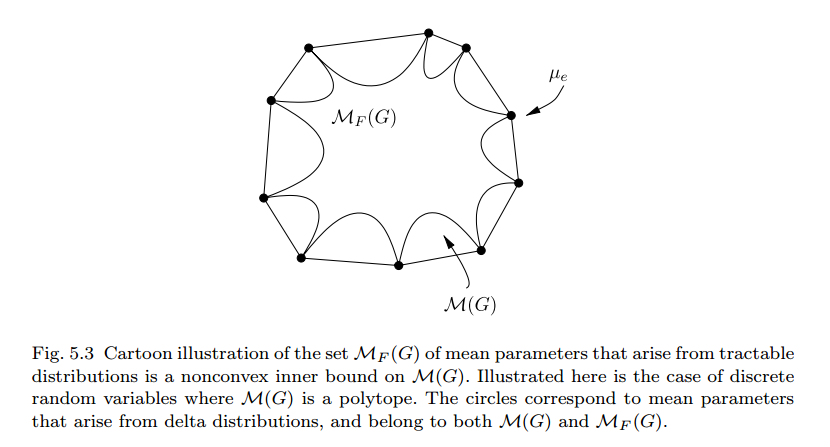
\includegraphics[scale = 0.45]{mean_field_region.png}}
\end{minipage}
\caption{\footnotesize{\textbf{The mean field parameter space $\cM_{\cF}(\cG)$ is an non-convex inner bound for $\cM(\cG)$.}}}
\label{fig: mean_field_region}
\end{figure}

An important fact about the \textbf{mean field} approach is that the variational problem \eqref{eqn: mean_field} may be \underline{\textbf{\emph{nonconvex}}}, so that there may be \textbf{local minima}, and the mean field updates can have multiple solutions. The source of this nonconvexity can be understood in different ways, depending on the formulation of the problem. See \citep{wainwright2008graphical} for detailed discussions. 

The geometric perspective on the set $\cM(\cG)$ and its inner approximation $\cM_{\cF}(\cG)$ reveals that more generally, mean field optimization is
  \underline{\emph{\textbf{always nonconvex}}} for \underline{\emph{\textbf{any exponential family}}} in which the state space $\cX^m$ is finite. This is becase $\cM(\cG) = \text{conv}(\phi_{\alpha}, \alpha \in \cI)$ is a \emph{\textbf{convex hull}} spanned by potentials and $\cM_{\cF}(\cG) \subset \cM(\cG)$ is a strict subset of $\cM(\cG)$. So it must be a nonconvex set. Figure \ref{fig: mean_field_region} illustrates their relationship.  

Consequently, \emph{nonconvexity} is an \emph{intrinsic property} of mean field approximations. 


\newpage
\bibliographystyle{plainnat}
\bibliography{book_reference.bib}
\end{document}